%! TeX program = lualatex
\documentclass[fleqn, twocolumn]{article}
\usepackage{amsfonts}
\usepackage{bm}
\usepackage{array, makecell}
\usepackage[x11names, table]{xcolor}
\usepackage{colortbl}
\usepackage{amsmath}
\usepackage{amsthm}
\usepackage{graphicx}
\usepackage{amssymb}
\usepackage{tabto}
\usepackage{verbatim}
\usepackage{hyperref}
\usepackage{enumitem}
\usepackage{listings}
\usepackage{xcolor}
\usepackage{fancyvrb}
\usepackage{algorithm}
\usepackage{algpseudocode}
\usepackage{calc}
\usepackage{emoji}
\usepackage[T1]{fontenc}
%\usepackage{mathptmx}
\usepackage{times}
\usepackage{graphicx}
\usepackage{tikz}
\usepackage{multicol}
\usetikzlibrary{graphs,graphdrawing,arrows.meta}
\usegdlibrary{trees}
\newcommand{\R}{\mathbb{R}}
\newcommand{\N}{\mathbb{N}}
\newcommand{\norm}[1]{\left\lVert#1\right\rVert}
\newcommand{\abs}[1]{\left\lvert#1\right\rvert}
\newcommand{\inner}[2]{\left\langle#1, #2\right\rangle}
\newcommand{\set}[1]{\left\{#1\right\}}
\newcommand{\grad}[1]{\nabla #1}
\newcommand{\hessian}[1]{\nabla^2 #1}
\newcommand{\expectation}[1]{\mathbb{E}\left[#1\right]}
\newcommand{\expectationwrt}[2][]{\mathbb{E}_{#2}\left[#1\right]}
\newcommand{\bigO}[1]{\mathcal{O}\left(#1\right)}

\author{Sharanshangar Muhunthan \\ \texttt{shangar.muhunthan@mail.utoronto.ca}}
\newtheorem{definition}{Definition}
\usepackage[margin=0.75in]{geometry}
\title{BOLT \emoji{high-voltage}: Bilateral Filtering and Octree Lightweight Technique for Fast and Parameter Free Point Cloud Upscaling}

\begin{document}
\maketitle
\begin{abstract}
	In this paper, we introduce BOLT (\underline{B}ilateral filtering and \underline{O}ctree \underline{L}ightweight \underline{T}echnique), a novel fast and parameter free method for upsampling point clouds.
	We leverage the structural efficiency of the octree data structure and detail preserving properties of the bilateral filter to achieve a fast and parameter free upsampling method.
	Unlike the current state-of-the-art methods, BOLT does not require any parameters, deep learning, fine tuning or any type of training making it a suitable candidate for real-time applications.
	BOLT understands the underlying structure of the point cloud by dividing the point cloud into a hierarchical octree structure. 
	Empty children are filled in the octree and outliers are smoothed using a bilateral filter.
	We evaluate BOLT on various point clouds and compare it with the current state-of-the-art methods and show competitive results.
\end{abstract}

\section{Introduction}

A pointcloud is an unordered 3D representation of a set of points in space.
It is commonly used in computer graphics, computer vision, and robotics.
Pointclouds are often generated using 3D scanners, LIDAR, and many more 3D applications.

In this work we wish to upsample a pointcloud. Given a set of point clouds, we wish to find a new set of points that are more dense but still represent the same underlying surface.
Further, the new points while preserving the underlying structure should not introduce any new artifacts, and should be informative and not clustered around the original points.
The unstructured and unordered nature of point clouds makes this a challenging problem. 
Further, existing methods for point cloud upsampling often are computationally expensive and require extensive training and parameter tuning. 

To address the above challenges we present a data-structure-driven method for point cloud upsampling that is fast and parameter free. 
Our method utilizes an octree data structure without a depth limit to understand the underlying structure and initially add points to the empty children of the octree.
The lack of a depth limit allows tighter fitting bounding cubes around points and allows for a more accurate representation of the underlying structure.
This representation is often noisy and coarse but captures the underlying structure of the point cloud. 
To smooth the point cloud, we use a bilateral filter in a point cloud application \cite{3d_bilateral_filter_ipol} to smooth the point cloud.

Point cloud upsampling can be used as a downstream task for various applications such as 3D reconstruction, 3D object recognition, and 3D rendering. 
It can be used to improve the quality of surface reconstruction, enhance object detection, extract features more accurately, and more. 

Our method, namely BOLT, learns the geometry and strucutre of the point cloud, upsamples and smooths it without any parameters, deep learning, or fine tuning.


\section{Related Work}

Many non-deep learning based methods for point cloud upsampling have been proposed in the past such as moving least squares interpolation (MLS interpolation) in 2002 \cite{Alexa2003ComputingAR},
Locally Optimal Projection (LOP) in 2007 \cite{LOP}, Edge Aware Resampling (EAR) in 2013 \cite{EdgeAwareResampling} and graph total variation in 2019 \cite{GraphTotalVariation}.

MLS works by fitting a continuous surface to a set of local points using a weighted least squares fit of a polynomial surface to the points. 
Points are added by computing the voronoi cells on the local surface and adding points to the vertices of the diagram.

LOP unlike MLS does not require fitting a local surface. Instead, it uses a projection operator to project points onto a surface in a way that minimizes the sum of the weighted distances between the original and projected points. Improvements to LOP such as weighted LOP \cite{WLOP} were proposed that make LOP more robust to noise and outliers. 

Both MLS and LOP have demonstrated good results but a common problem with these methods is they don't perform well on sharp edges and corners, as the model often assumes a smooth surface.

EAR was designed to work well on edges \cite{EdgeAwareResampling}. 
It works by first computing the normals and relateive curvature of each point.
Then if the curvature is above a certain threshold, the point is considered to be on an edge, and the point is projected onto the tangent plane of the edge.
If a point is considered a surface, the point is projected onto the tangent plane of the surface.

Graph total variation is a method that uses a graph to represent the point cloud. 
They first construct a triangular mesh, then insert points at the centroids of the triangles. 
Assuming the point cloud is piecewise smooth, they then minimize a weighted average of the $L_1$ norms 
of normals between points.

Many deep learning based approaches also exist, such as PU-Net \cite{PU-Net}, PU-GAN \cite{PU-GAN} and PU-GCN \cite{PU-GCN}. Although these point cloud upsampling methods tackle a different problem, they were still used as a point of comparison.
The reason these are solving different problems is because these are large networks trained on large datasets, and require a lot of computational power to train and run. The goal of this paper is to propose a fast and parameter free method for point cloud upsampling.


\section{Background}

\subsection{Octree}

An octree is a tree data structure in which each internal node has exactly eight children. 
Octrees are often used to partition 3D space and are used in various applications such as computer graphics, computer vision, and robotics.

\begin{figure}[H]
	\centering
	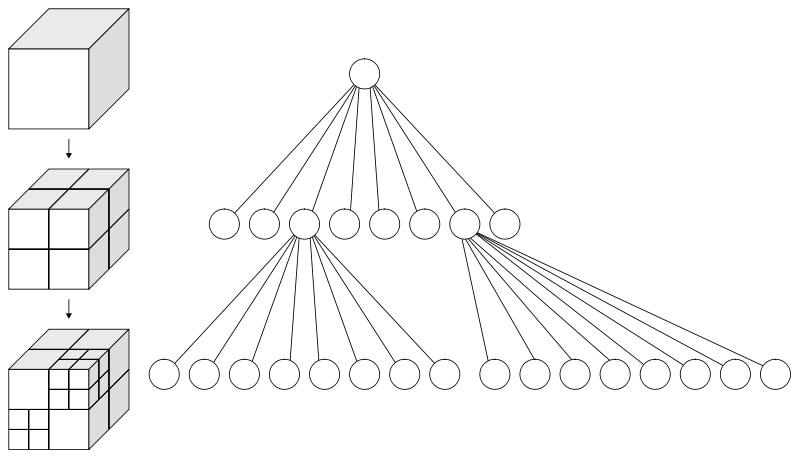
\includegraphics[width=0.5\textwidth]{octree.png}
	\caption{An example of an octree. Each cube gets recursively divided into eight equal octants. The points are stored in the leaf nodes. Image from \cite{octree_diagram}}
	\label{fig:octree}
\end{figure}

In the context of point clouds, an octree is used to partition the 3D space and store the points in the leaf nodes.
The octree is a hierarchical data structure that recursively divides 3D space into eight equal octants.
Each node in the octree represents a rectangular prism in 3D space with a particular center, width, lenghth and depth.
Nodes that aren't leaf nodes have exactly eight children, and leaf nodes store the points in the point cloud.
The root node of the octree represents the bounding box of the point cloud.
An octree has $\bigO{\log n}$ complexity for insertion and search operations, where $n$ is the number of points in the point cloud.
Bounding cubes nearest points are much finer and tighter fitting than those further away, allowing for a more accurate representation of the underlying structure of the point cloud.

Further, these tighter bounding boxes give hints on where to add new points to the point cloud, since adding points to the tighter bounding boxes will result in points that are more informative and not clustered around the original points, will not introduce any new artifacts, and will preserve the underlying structure of the point cloud.

Most octrees have a depth limit, which means that the octree will not divide the space beyond a certain depth, this is to avoid a problem of infinite recursion.
However, in our method, we do not have a depth limit, and we allow the octree to divide the space as much as possible.
since the starting point clouds are often sparse and noisy, and the lack of a depth limit allows for a more accurate representation of the underlying structure of the point cloud.
Other stops such as checking if an existing close point is already in the node are used to avoid infinite recursion.


\begin{figure}[H]
	\centering
	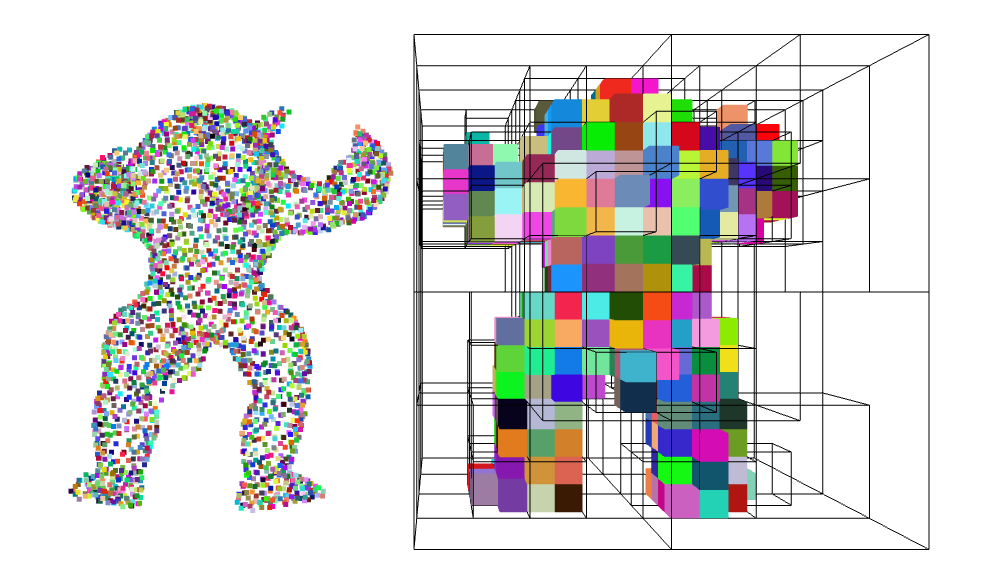
\includegraphics[width=0.5\textwidth]{octree_demo.png}
	\caption{An example of an octree with its point cloud and cubed representation. The figure was from a blog post \cite{octree_demo} and was generated using the Open3D library \cite{open3d} with a max depth of 4.}
	\label{fig:octree_depth}
\end{figure}

\subsection{Bilateral Filter}

The bilateral filter is a non-linear filter that is used to smooth images and reduce noise while preserving edges.
It is a generalization of the Gaussian filter, and it is used in various applications such as image processing, computer graphics, and computer vision.
It is defined as follows:
$$ B(I, x) = \sum\limits_{x_i \in \Omega} I(x_i) f_r(\norm{x_i - x})g_s(\norm{x_i - x})$$

In our paper, we use the bilateral filter to smooth the point cloud. Similar to the image case, the bilateral filter smooths the point cloud while preserving the edges and the underlying structure of the point cloud. It works by shifting points along a normal vector, and the amount of shift is a weighted average distance to its neighbours.
We follow Digne et al. \cite{3d_bilateral_filter_ipol} and use the following definition of the bilateral filter for point clouds:

\begin{equation} p' = p + \delta_p \cdot n_p\end{equation} 

Where $n_p$ is the normal to the regression plane of some $k$ nearest neighbours of $p$. Also following Dinge et al \cite{3d_bilateral_filter_ipol}, our implementation computes the normal with PCA. PCA will find the regression plane that fits the data best and the corresponding found eigenvectors will be orthogonal to said plane, and thus is simple to compute compared to an iterative least squares method. $\delta_p$ is the displacement of the point $p$.
The displacement is computed as follows, let $\mathcal{N}_p$ be the set of $k$ nearest neighbours of $p$:

\begin{equation}\label{eq:delta}  \delta_p = \dfrac{\sum\limits_{q \in \mathcal{N}_p} w_d(\norm{q - p})w_n(\inner{n_p}{q-p})\inner{n_p}{q-p}}{\sum\limits_{q \in \mathcal{N}_p}w_d(\norm{q - p})w_n(\inner{n_p}{q-p})}\end{equation} 

In our implementation, $w_d$ and $w_n$ are the Gaussian functions defined as follows:

\begin{equation} w_i(x) = \exp\left\{-\dfrac{x^2}{2\sigma_i^2}\right\} \label{eq:weight}\end{equation} 

In our implementation we set $\sigma_d = 0.1$ and $\sigma_n = 0.1$.


\section{Methodology}

Our goal is to upscale and then smooth a sparse point cloud using an octree with a large depth and bilateral filtering on a point cloud.
We start with a sparse point cloud $\mathcal{P} = \{p_1, \dots, p_n\}$, and generate an octree $\mathcal{T}$ by iterating through and inserting one at a time.
To generate the initial upsampling of the points, we find the parent of each for point $p_i$ in $\mathcal{T}$, 
then add a new point to an empty child of the parent in $\mathcal{T}$. 
One such iteration will double the number of points in the point cloud, then another will quadruple and so on. 
This process gets repeated the number of times necessary to get the desired final number of points.
Then we extract all points from $\mathcal{T}$ to get our new upsampled point cloud $\mathcal{P}'$.
We then smooth $\mathcal{P}'$ with bilateral filtering. Bilateral filtering requires hyper parameters $\sigma_d, \sigma_n$ and $k$. $k$ indicates the number of neighbours used to find the normal of the regression plane, and $\sigma_d, \sigma_n$ are the standard deviations for the gaussians used in (\ref{eq:weight}).

\begin{algorithm}[H]
	\caption{Main upsampling algorithm}
	\begin{algorithmic}
		\Require sparse point cloud ${P}$ with $n$ points, $n_{\text{up}}$ number of iterations required to get the desired number of points 
		\Function{upsample}{{P}}
		\State {T} \gets \Call{constructOctree}{{P}}
		\State $P_n$ \gets \Call{EmptyPointCloud}{}
		\For{$i \leq n_{\text{up}}$}
			\For{$p \in P$}
				\State parent \gets $p$.parent 
				\State child \gets \Call{randomEmptyChild}{parent}
				\State $p'$ \gets \Call{randomPointInside}{child.dimensions}
				\State \Call{insert}{$p'$, $P_n$}
			\EndFor
		\EndFor
		\State P \gets \Call{convertToPointCloud}{T}
		\State \Call{bilateralSmooth}{P, $P_n$}
		\EndFunction
	\end{algorithmic}
\end{algorithm}

\begin{algorithm}[H]
	\caption{Bilateral smoothing algorithm, borrowed heavily from \cite{3d_bilateral_filter_ipol}}
	\begin{algorithmic}
		\Require point cloud ${P}$ with $n$ points, $P_n$ new points, $k$ neighbours, $\sigma_d$, $\sigma_n$
		\Function{bilateralSmooth}{{P}, $P_n$}
		\For{$p \in P_n$}
			\State $\mathcal{N}_p$ \gets \Call{findNeighbours}{P, k, p}
			\State $\textbf{n}_p$ \gets \Call{computeUnitNormalToPlane}{$\mathcal{N}$}
			\State $s_w$ \gets 0
			\State $\delta_p$ \gets 0
			\For{$q \in \mathcal{N}_p$}
			\State $w$ \gets $w_d(\norm{p - q}) \cdot w_n(\inner{\textbf{n}_p}{p - q})$ \Comment{From (\ref{eq:weight})} 
				\State $s_w$ \gets $s_w + w$
				\State $\delta_p$ \gets $\delta_p + w \cdot \inner{\textbf{n}_p}{p - q}$
			\EndFor
			\State $p'$ \gets $p + \frac{\delta_p}{s_w} \cdot \textbf{n}_p$
		\EndFor
		\EndFunction
	\end{algorithmic}
\end{algorithm}



\section{Experiments}

Experiments were done mostly with the ShapeNet dataset \cite{shapenet}, which is a large dataset of 3D models. 
A random set of either 1024 point clouds were sampled and then upscaled to double or 2048 points.
We then compare use some evaluation metrics with the ground truth to see how well our method performs in a quantitative manner.
In the appendix we highlight the qualitative results of our method compared to other methods used in this paper.


\subsection{Evaluation}

We will eventually evaluate our model using the Chamfer distance and Hausdorff distance as they are common metrics used in point cloud upsampling, and try to compare to other parameter free works as well as deep learning based methods.
The Chamfer distance is a measure of how different 2 shapes are and is defined as the following:

$$ C(P, Q) = \dfrac{1}{|P|} \sum\limits_{p \in P} \min_{q \in Q} \norm{p - q}^2 +  \dfrac{1}{|Q|} \sum\limits_{q \in Q} \min_{p \in P} \norm{p - q}^2 \label{eq:chamfer}$$

The Hausdorff distance is a measure of how similar 2 sets are. It is defined as the following:

$$ H(A, B) = \max(h(A, B), h(B, A))\label{eq:hausdorff}$$

Where:

$$h(A, B) = \max_{a \in A} \min_{b \in B} \norm{a - b}$$

In terms of comparisons, we perform comparisons with MLS as a baseline for another non-deep learning based method, as well as with PU-GCN as a deep learning based method.
We also see how our method performs compared to other smoothing methods such as KNN and no smoothing, as well as different sampling methods such as random sampling and octree sampling.
This is to show that our choices in smoothing and sampling are the best in this context.

\subsection{Comparison with Non-Deep Methods}

We compared our results with MLS, which is a non-deep learning based method of upsampling point clouds using local surface fitting.

\begin{table}[H]
\centering
\begin{tabular}{ccc}
	& Chamfer distance $\times 10^3$ &\\
	\hline
	class & MLS & Ours \\
	\hline
	plane & \textbf{14.8} & 15.8 \\ 
	helmets & \textbf{26.7} & 29 \\
	cap & \textbf{22.4} & 24.4 \\  
	car & \textbf{28.6} & 31 \\  
	headset & {25.3} & \textbf{23.8}  \\
\end{tabular}
\caption{Comparison of our method with MLS with chamfer distance $\times 10^3$. Note that lower is better}
\end{table}

\begin{table}[H]
\centering
\begin{tabular}{ccc}
	& Hausdorff distance $\times 10^3$ &\\
	\hline
	class & MLS & Ours \\
	\hline
	plane & 282.9 & \textbf{80.5} \\ 
helmets & 454.8 &  \textbf{182.2}\\
cap & \textbf{150.2} & 156.3 \\ 
car & 75.3 & \textbf{73.5} \\  
headset & 171.3 & \textbf{166.5} \\
\end{tabular}
\caption{Comparison of our method with MLS with Hausdorff distance $\times 10^3$. Note that lower is better}
\end{table}

In general, our method performed better than MLS in terms of the Hausdorff distance, but worse in terms of the Chamfer distance.
In some cases, our method performed better in both metrics, such as the headset class.
In terms of execution time, we found that our method was also slower than MLS, taking 0.5 seconds to run in total compared to 0.2 seconds for MLS.
Note however that the MLS implementation was written entirely in C++. Our method only implements the bilateral filter in C++ and the rest in Python. 
This difference in overhead may account for the difference in execution time.

A worse chamfer distance but better hausdorff distance indicates that our method is better at preserving global shape, but worse at preserving local shape.
It also implies that our method is better at preserving the overall structure of the point cloud, but worse at preserving the details, and also implies that our method is less sensitive to outliers than MLS.
This sensitivity to outliers for MLS can be reflected in the car example in the appendix, where the MLS method has few points that are very far from the shape, where as our method does not have this issue.

Overall depending on the task at hand, one may choose to use MLS or our method. If the task requires preserving the overall structure of the point cloud, our method is better. If the task requires preserving the details of the point cloud, MLS is better.

\subsection{Comparison of Other Smoothing Methods}

We compared our method with other smoothing methods, such as the bilateral filter and a K-nearest neighbors based method as well as no smoothing and just the octree sampling.

\begin{table}[H]
\centering
\begin{tabular}{cccc}
	&  & Chamfer distance $\times 10^3$ &\\
	\hline
	class & KNN & Bilateral & None\\
	\hline
	plane & {16.2} & \textbf{15.8} & {16} \\ 
	helmets & {29.3} & \textbf{29} & {29.8} \\
	cap & {24.5} & \textbf{24.4} & {25.5}\\  
	car & {31.3} & \textbf{31} & \textbf{31}\\  
	headset & {24.4} & \textbf{23.8} & {24.2} \\
\end{tabular}
\caption{Comparison of our method with MLS with chamfer distance $\times 10^3$. Note that lower is better}
\end{table}

\begin{table}[H]
\centering
\begin{tabular}{cccc}
	&  & Hausdorff distance $\times 10^3$ &\\
	\hline
	class & KNN & Bilateral & None\\
	\hline
	plane & 81.3 & {80.5} & \textbf{78.4} \\ 
	helmets & 186.2 &  {182.2} & \textbf{182.1}\\
	cap & \textbf{149.4} & {156.3} & {155.6}\\ 
	car & \textbf{72.1} & {73.5} & {74}\\  
	headset & 168.3 & \textbf{166.5} & \textbf{166.5}\\
\end{tabular}
\caption{Comparison of our method with MLS with Hausdorff distance $\times 10^3$. Note that lower is better}
\end{table}

In general, our method performed better than the KNN method in terms of both the Chamfer and Hausdorff distance, with the exception of the cap and car classes. 
Bilateral also performed better than no smoothing in terms of Chamfer distance, but worse in terms of the Hausdorff distance.

\subsection{Comparison of Different Sampling Methods}

In this subsection we compare our octree sampling method with random sampling, both cases using bilateral smoothing.

\begin{table}[H]
\centering
\begin{tabular}{ccc}
	& Chamfer distance $\times 10^3$ &\\
	\hline
	class & Random & Octree \\
	\hline
	plane & {49.1} & \textbf{15.8} \\ 
	helmets & {40} & \textbf{29} \\
	cap & {38.7} & \textbf{24.4} \\  
	car & {36.7} & \textbf{31} \\  
	headset & {46} & \textbf{23.8}  \\
\end{tabular}
\caption{Comparison of our method with random sampling with chamfer distance $\times 10^3$. Note that lower is better}
\end{table}

\begin{table}[H]
\centering
\begin{tabular}{ccc}
	& Hausdorff distance $\times 10^3$ &\\
	\hline
	class & Random & Octree \\
	\hline
	plane & 86.2 & \textbf{80.5} \\
	helmets & \textbf{172.4} &  {182.2}\\
cap & \textbf{153.4} & {156.3} \\
car & {74.6} & \textbf{73.5} \\
headset & 178.3 & \textbf{166.5} \\
\end{tabular}
\caption{Comparison of our method with random sampling with Hausdorff distance $\times 10^3$. Note that lower is better}
\end{table}

Clearly, the octree sampling method outperforms the random sampling method in terms of Chamfer distance, but slightly better in terms of the Hausdorff distance.
This shows that using an octree to voxelize and add points nearby points is a better method than randomly sampling points.

\subsection{Comparison with Deep Methods}

We will compare our method with deep learning based method PU-GCN\cite{PU-GCN}.
First, an analysis of the computational cost of using PU-GCN will be done. 
When experimenting with an Nvidia 4090, we found that the PU-GCN took 10GB of memory during training.
We trained the PU-GCN model for 10 epochs, which took 2 hours to train.
The original paper trained the model for 100 epochs. 
This is a significant amount of time and memory, and is a disadvantage of the PU-GCN method.
In the PU-GCN paper they authors claimed a chamfer distance of $\sim 0.5 \times 10^3$ and a Hausdorff distance of $\sim 1 \times 10^3$.
This is much lower than our method, but the computational cost is much higher.
This is also much lower than what we found in our experiments but is likely due to the fact that we only trained for 10 epochs.
This comparison was done with the PU1K dataset. Each point cloud was a sample of 256 points and was upsampled to 1024 points. 

\begin{table}[H]
\centering
\begin{tabular}{ccc}
	& Hausdorff $\times 10^3$ &\\
	\hline
	class & PU-GCN & Ours \\
	\hline
	eight & \textbf{96.1} & {221.3} \\ 
	elephant &  \textbf{74.1}& {122.6} \\
	elk & {94.6} & \textbf{52} \\  
	fandisk & \textbf{86} & {169.3} \\  
	genus3 & \textbf{127.1} & {378.6}  \\
\end{tabular}
\caption{Comparison of our method with PU-GCN with chamfer distance $\times 10^3$. Note that lower is better}
\end{table}

Our method does much worse in terms of the Hausdorff distance.
However, the computational cost of our method is much lower than PU-GCN.




\section{Conclusion}

In conclusion, this paper presents BOLT, a novel fast and parameter free method for upsampling point clouds.
Our method leverages the structural efficiency of the octree data structure and detail preserving properties of the bilateral filter to achieve a fast and parameter free upsampling method.
Unlike the current state-of-the-art deep methods, BOLT does not require any parameters, deep learning, fine tuning, GPU or any type of training making it a suitable candidate for real-time applications.
We evaluate BOLT on various point clouds and compare it with the current state-of-the-art methods and show competitive results.
In future work, we plan to implement BOLT in C++ and add concurrency to reduce the overhead and improve the execution time.


\bibliographystyle{plain}
\bibliography{refs}

\end{document}
